\section{Introduction}
\label{sec:intro}

We present Nemotron 3 Ultra, the largest and most capable model in the Nemotron 3 family~\citep{blakeman2025nvidia}. As LLM applications evolve from simple chatbots to long-running agents capable of autonomously writing code, conducting research, and completing complex tasks, the ability to deliver fast and efficient inference becomes increasingly important. Nemotron 3 Ultra addresses this by employing a Mixture-of-Experts hybrid Mamba-Attention architecture, leading to improvements along the inference-throughput-to-accuracy frontier. While Mixture-of-Experts help Nemotron 3 Ultra achieve better accuracy per active parameter, the hybrid Mamba-Attention architecture significantly improves inference throughput by reducing attention cost and KV cache footprint. Nemotron 3 Ultra achieves 5.9$\times$, 4.8$\times$, and 1.6$\times$ higher inference throughput compared to GLM-5.1-754B-A40B, Kimi-K2.6-1T-A32B, and Qwen-3.5-397B-17B respectively on 8K input / 64K output token setting while also attaining on-par accuracy across a wide range of agentic and reasoning benchmarks.


\begin{figure}[ht]
    \centering
    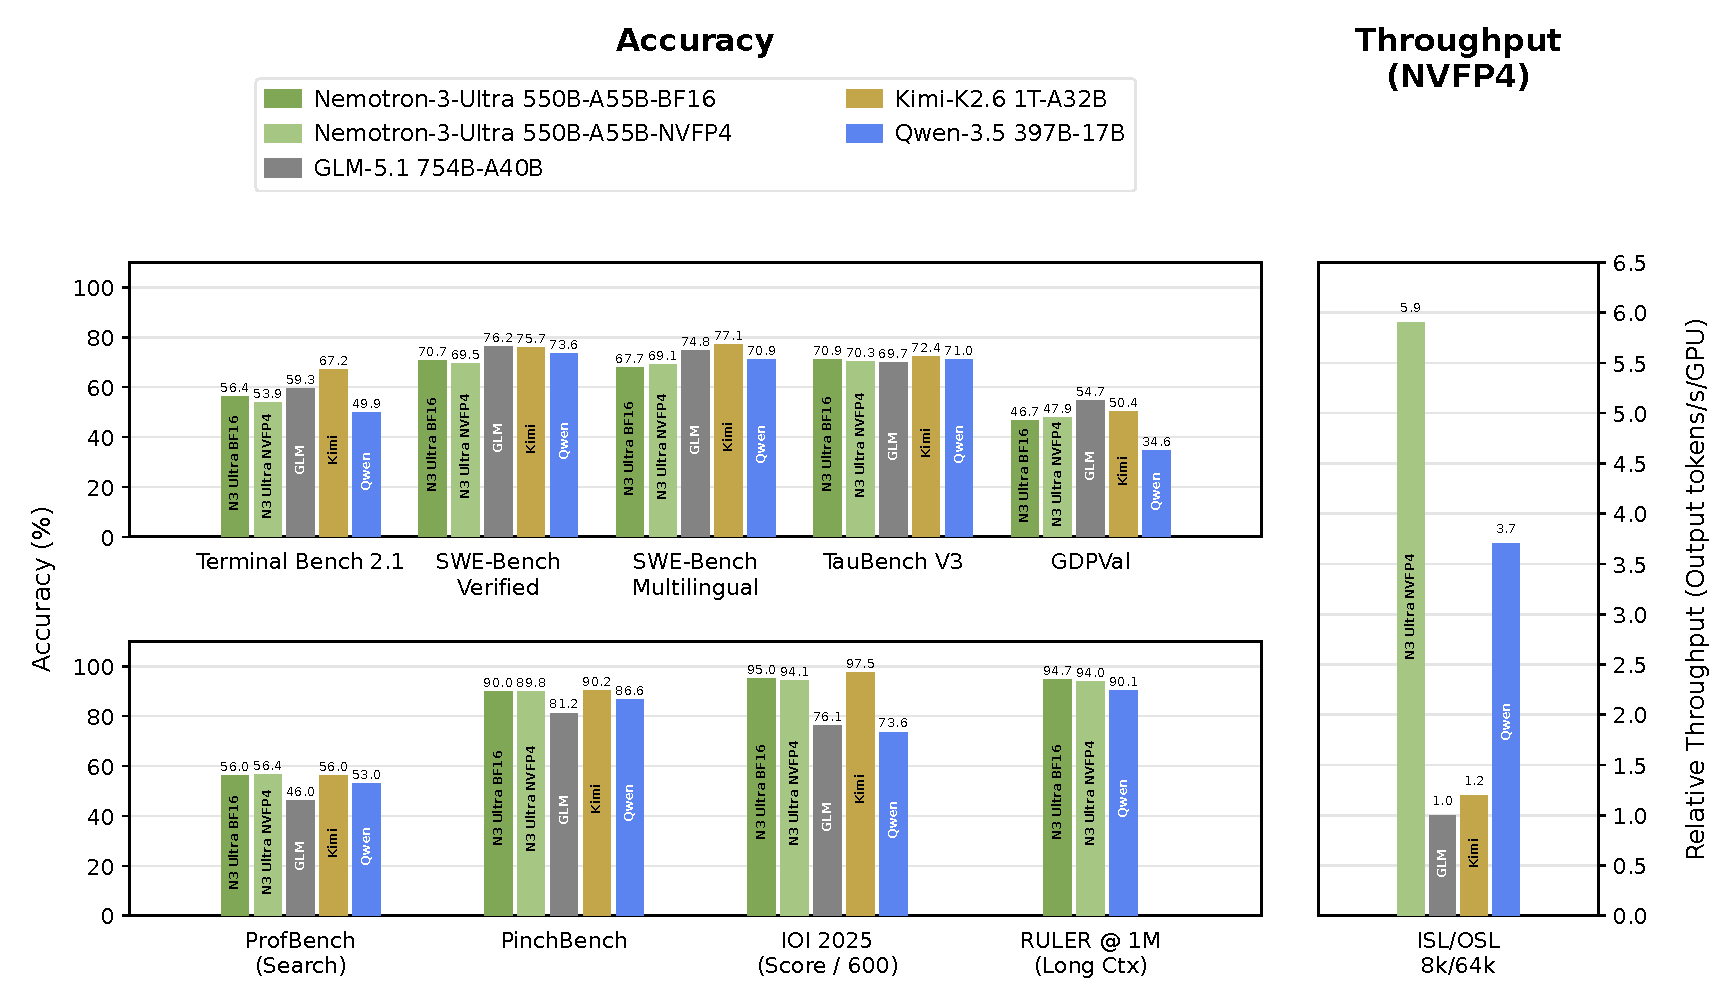
\includegraphics[width=\linewidth]{figures/ultrav3-comp.pdf}
    \caption{Accuracy and throughput comparisons for \ourmodel. Our model achieves on-par accuracy with other open LLMs while achieving significantly higher inference throughput on the 8K input / 64K output token setting. All throughput numbers are reported at max-throughput using NVFP4 precision on GB200. For Nemotron 3 Ultra, throughput numbers are obtained from TRT-LLM, while all other model numbers use vLLM. We run with and without speculative decoding, where available, and choose the best numbers for each model.}
    \label{fig:intro}
\end{figure}


We pretrained \ourbasemodel with all the key Nemotron 3 features and technologies~\citep{blakeman2025nvidia}, including NVFP4 pre-training, LatentMoE~\citep{latentmoe_tr}, and Multi Token Prediction (MTP)~\citep{gloeckle2024better}. We pretrained our base model in NVFP4 with 20 trillion text tokens using a Warmup-Stable-Decay learning rate schedule. Pretraining was divided into two phases with 15 trillion tokens of data in the first phase focusing on diversity and broad domain coverage followed by 5 trillion tokens of data in the second phase focusing on high quality data to refine model accuracy. LatentMoE helped us achieve better accuracy per parameter than standard Granular MoEs~\citep{dai2024deepseekmoe} while Multi Token Prediction (MTP) leads to faster inference with speculative decoding. Our pretrained base model achieves significantly higher accuracy than other publicly available base models, such as DeepSeek v3.2~\citep{deepseekai2024deepseekv32}, Mistral Large 3, Kimi-K2~\citep{kimiteam2025kimik2openagentic}, and GLM-4.5~\citep{5team2025glm45agenticreasoningcoding}.

We trained \ourmodel with an agent-focused post-training pipeline to improve its long-horizon reasoning, tool use, and autonomous task completion capabilities. The initial SFT stage used a carefully curated data mixture to build the model's foundational capabilities. This was followed by unified RLVR over a wide mix of reasoning, agentic, code, safety, usability, and chat environments. In parallel, more than ten domain-specialized teacher models were trained using targeted recipes, including agentic teachers built on a dedicated agentic SFT path. Finally, Multi-teacher On-Policy Distillation (MOPD) consolidated these teachers into Ultra through dense token-level guidance on student-generated rollouts. Ultra is also equipped with reasoning effort control, which supports inference-time adjustment of the accuracy–compute trade-off.

We are releasing the Base, Post-Trained, and NVFP4 quantized checkpoints on HuggingFace. Alongside the checkpoints, we are also open-sourcing the training recipes\footnote{\href{https://github.com/NVIDIA-NeMo/Nemotron}{https://github.com/NVIDIA-NeMo/Nemotron}}, data, and RL environments. 

\paragraph{Checkpoints}
\begin{itemize}
    \item \href{https://huggingface.co/nvidia/NVIDIA-Nemotron-3-Ultra-550B-A55B-NVFP4}{\texttt{Nemotron 3 Ultra 550B-A55B NVFP4} 
\includegraphics[height=0.9em]{assets/huggingface-color.png}} : post-trained and NVFP4 quantized model
    % \item \href{https://huggingface.co/nvidia/NVIDIA-Nemotron-3-Super-120B-A12B-FP8}{\texttt{Nemotron 3 Super 120B-A12B FP8} 
\includegraphics[height=0.9em]{assets/huggingface-color.png}} : post-trained and FP8 quantized model
    \item \href{https://huggingface.co/nvidia/NVIDIA-Nemotron-3-Ultra-550B-A55B-BF16}{\texttt{Nemotron 3 Ultra 550B-A55B BF16} 
\includegraphics[height=0.9em]{assets/huggingface-color.png}} : post-trained model
    \item \href{https://huggingface.co/nvidia/NVIDIA-Nemotron-3-Ultra-550B-A55B-Base-BF16}{\texttt{Nemotron 3 Ultra 550B-A55B Base BF16} 
\includegraphics[height=0.9em]{assets/huggingface-color.png}} : base model
    \item \href{https://huggingface.co/nvidia/NVIDIA-Nemotron-3-Ultra-550B-A55B-GenRM}{\texttt{Nemotron 3 Ultra 550B-A55B GenRM} 
\includegraphics[height=0.9em]{assets/huggingface-color.png}} : GenRM used for RLHF

\end{itemize}

\paragraph{Data}
\begin{itemize}
    \item \href{https://huggingface.co/datasets/nvidia/Nemotron-Pretraining-Code-v3}{\texttt{Nemotron-Pretraining-Code-v3} 
\includegraphics[height=0.9em]{assets/huggingface-color.png}} : 173B tokens of fresh code data from GitHub through September 30, 2025.
    \item \href{https://huggingface.co/datasets/nvidia/Nemotron-Pretraining-Legal-v1}{\texttt{Nemotron-Pretraining-Legal-v1} 
\includegraphics[height=0.9em]{assets/huggingface-color.png}} : A collection of synthetic datasets intended to improve the legal capabilities of LLMs. In one ablation, adding these datasets to Nemotron 3 Nano pretraining boosted a proxy LegalBench average accuracy from 64.6 to 74.7.
    \item \href{https://huggingface.co/datasets/nvidia/Nemotron-Pretraining-Specialized-v1.2}{\texttt{Nemotron-Pretraining-Specialized-v1.2} 
\includegraphics[height=0.9em]{assets/huggingface-color.png}} : A collection of synthetic datasets aimed to improve LLM capabilities on factual recall, moral scenarios, and diverse generative and multiple choice questions.
    \item \href{https://huggingface.co/collections/nvidia/nemotron-post-training-v3}{\texttt{Nemotron-Posttraining-v3} 
\includegraphics[height=0.9em]{assets/huggingface-color.png}} : A collection of post-training datasets for improving agentic, reasoning, and general model capabilities during SFT and RL.
\end{itemize}

% \newparagraph{Artifacts}
% \begin{itemize}
% \end{itemize}



We organize the remainder of the report into 4 sections: Pretraining~(\S\ref{sec:pretraining}), Post-training~(\S\ref{sec:posttraining}), Quantization~(\S\ref{sec:quantization}), and Inference~(\S\ref{sec:inference}).